\documentclass[12pt]{amsart}
\usepackage[left=0.5in, right=0.5in, bottom=0.75in, top=0.75in]{geometry}
\usepackage[english]{babel}
\usepackage[utf8x]{inputenc}
\usepackage{amsmath,amssymb,amsthm}
\usepackage{enumerate}
\usepackage{graphicx}


\usepackage[dvipsnames]{xcolor}
\usepackage{xparse}
\usepackage{tikz}
\usepackage{pgfplots}
\usepgfplotslibrary{fillbetween}

\renewcommand{\thesection}{}
\renewcommand{\thesubsection}{\arabic{subsection}}
\renewcommand{\thesubsubsection}{\quad(\alph{subsubsection})}

\begin{document}
\raggedbottom

\noindent{\large OPER 618 - Game Theory and Math Programming %
	- Homework 6 }
\hspace{\fill} {\large B. Hosley}
\bigskip


%%%%%%%%%%%%%%%%%%%%%%%
\setcounter{subsection}{0}
\subsection{}
\textbf{Bilevel Programming Problems.} 
\textit{Consider the following linear BLPP.}
\begin{align*}
	\min_x\	\ x &+ 3y \\
	\text{s.t. }\	1 &\leq x \leq 6 \\
	y \in \arg\min \{ -y &: x + y \leq 8, x + 4y \geq 8, x + 2y \leq 13 \}
\end{align*}

\subsubsection{}
\textit{Draw the relaxed feasible region $\Omega$.} \\
 
The gray shaded area represents the relaxed feasible area. 

%
% neg gradient is the direction of greatest improvement for the minimize problem
%

\begin{center}
	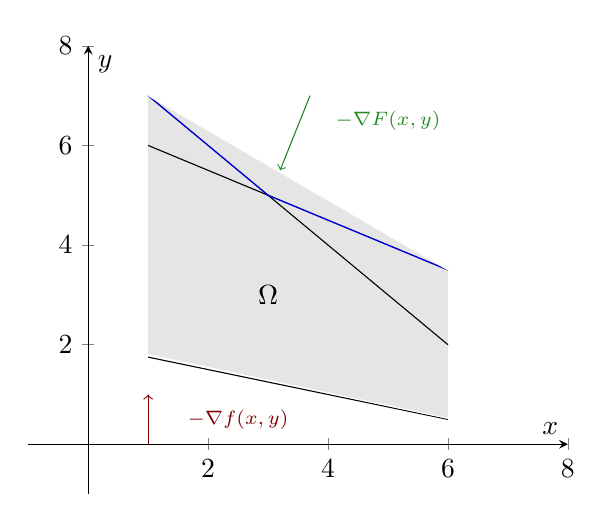
\begin{tikzpicture}
		\begin{axis}[xmin=-1, xmax=8, ymin=-1, ymax=8, axis x line=middle, axis y line=middle, ylabel=$y$, xlabel=$x$]
			\addplot[domain=1:6]{8-x}; 		% x + y <= 8
			\addplot[domain=1:6]{2-x/4};	% x + 4y >= 8
			\addplot[domain=1:6]{6.5-x/2};	% x + 2y <= 13
			% Colored parts
			\addplot[domain=1:3, color=blue]{8-x}; 		% x + y <= 8
			\addplot[domain=3:6, color=blue]{6.5-x/2};	% x + 2y <= 13
			% Relaxed Feasible
			\addplot [name path=A, black!1] coordinates {(1,7) (6,3.5) };
			\addplot [name path=B, black!1] coordinates {(1,1.8) (6,0.52) };
			\addplot [gray!20] fill between[ of= A and B ];
			\node at (axis cs:3,3) {$\Omega$};
			% Follower gradient
			\addplot[->, color=Maroon] coordinates {(1,0) (1,1)};
			\node at (axis cs:2.5,0.5) {\scriptsize\textcolor{Maroon}{$-\nabla f(x,y)$}};
			% Leader gradient
			\addplot[->, color=ForestGreen] coordinates { (3.7,7) (3.2,5.5) }; % 0.5, 1.5
			\node at (axis cs:5,6.5) {\scriptsize\textcolor{ForestGreen}{$-\nabla F(x,y)$}};
		\end{axis}
	\end{tikzpicture}
\end{center}

\subsubsection{}
\textit{Somewhere on the plot, depict $-\nabla f(x,y)$, the negative of the gradient for the follower’s objective function.} \\

	The $-\nabla f(x,y) = \begin{bmatrix} 0 & 1 \end{bmatrix}$. It can be seen in \textcolor{red}{red} in the graph.

\subsubsection{}
\textit{Based on your answers to (a) and (b), draw the inducible region IR.} \\
	
	The inducible region is the \textcolor{blue}{blue} line(s) at the top of the feasible region.
		
\subsubsection{}
\textit{Somewhere on the plot, depict $-\nabla F(x,y)$, the negative of the gradient for the leader’s objective function.} \\
	
	The $-\nabla F(x,y) = \begin{bmatrix} -1 & -3 \end{bmatrix}$. It can be seen in \textcolor{green}{green} in the graph.
	
\subsubsection{}
\textit{Based on your answers on (c) and (d), what is the optimal decision for the leader?} \\

	Player one should select $x=6$. Player 2's best move would be $y=3.5$ resulting in $F(x,y) = 16.5$ and $f(x,y) = 3.5$. 
	
\clearpage

\subsection{}
\textbf{Bilevel Programming Problems.} 
\textit{Discuss how the complexity of solving the BLPP in Problem 1 would change under the following conditions. A written description is necessary, and a manual sketch to illustrate any points might be helpful.}

% 
% opt/pessimistic occurs when follower has multiple optima
% 

\subsubsection{}
\textit{The formulation included nonlinear constraints and/or nonlinear objective functions.} \\

Non-linear constraints will also require relaxation regardless of convexity of the move space.
Such that the entirety of the nonlinear area would be entirely include. 
A non-linear objective function presents a greater challenge. 
The gradient can still be calculated by iteratively integrating until a vector is returned.

\subsubsection{}
\textit{The formulation included integer restrictions on the leader and/or follower’s decision variables.} \\

Integers would similarly require relaxation, however, the domains previously applied will still work.
The last step in solving this problem will be to round the optimal point to integer.
Multiple integer pairs may need to be evaluated.

\subsection{}
\textbf{BLPPs – Optimistic and Pessimistic Solutions.} 
\textit{Consider the following BLPP, for which $y\in R(x)$ is not always a singleton.}

\begin{align*}
	\min_x	-x-y & \\
	\text{s.t.}\quad\	x \leq& 5 \\
	\min_y (-&|y|) \\
	\text{s.t.}\quad &	x^2 + y^2 \leq 16
\end{align*}

% 
% draw inducible region/ and the follower's neg gradient
% 

\subsubsection{}
\textit{Draw the relaxed feasible region $\Omega$.}

\begin{center}
	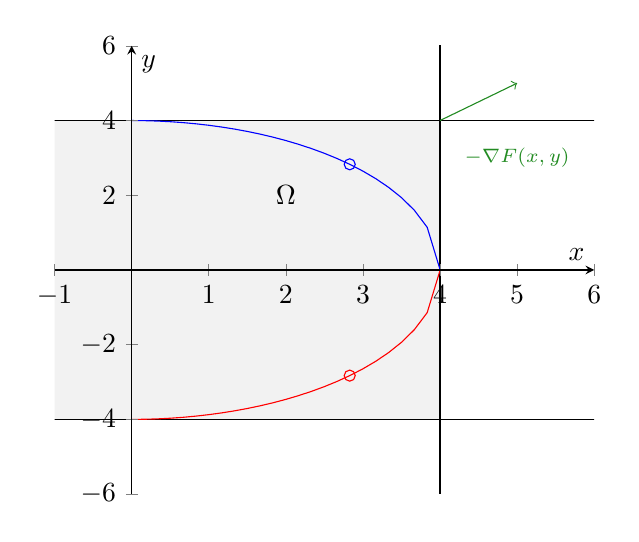
\begin{tikzpicture}
		\begin{axis}[xmin=-1, xmax=6, ymin=-6, ymax=6, axis x line=middle, axis y line=middle, ylabel=$y$, xlabel=$x$,axis on top]
			% Relaxed Feasible
			\addplot [domain=-2:8]{4}; 
			\addplot [domain=-2:8]{-4}; 
			\addplot [] coordinates {(4,8) (4,-6) };
			\addplot [name path=A] coordinates {(4,4) (4,-4) };
			\addplot [name path=B, black!1] coordinates {(-2,4) (-2,-4) };
			\addplot [gray!10] fill between[ of= A and B ];
			\node at (axis cs:2,2) {$\Omega$};
			% Colored parts
			\draw[thick] (axis cs:0,0) circle[radius=400];
			\addplot[domain=0:4, color=blue]{sqrt(16-x^2)};
			\addplot[domain=0:4, color=red]{-sqrt(16-x^2)};  	
			% Leader gradient
			\addplot[->, color=ForestGreen] coordinates { (4,4) (5,5) }; % 0.5, 1.5
			\node at (axis cs:5,3) {\scriptsize\textcolor{ForestGreen}{$-\nabla F(x,y)$}};
			% Solutions
			\addplot[red,mark=o] coordinates {( 2.828427, -2.828427 )};
			\addplot[blue,mark=o] coordinates {( 2.828427, 2.828427 )};
		\end{axis}
	\end{tikzpicture}
\end{center}


\subsubsection{}
\textit{Based on your answers to (a) and (b), draw the inducible region IR.} \\

	Once again, the relaxed area is shown as a gray shaded area.
	The optimistic inducible region is depicted in \textcolor{blue}{blue}, and the pessimistic region as \textcolor{red}{red}.

\subsubsection{}
\textit{Somewhere on the plot, depict $-\nabla F(x,y)$, the negative of the gradient for the leader’s objective function.} \\

	The $-\nabla F(x,y) = \begin{bmatrix} -1 & -3 \end{bmatrix}$. It can be seen in \textcolor{green}{green} in the graph.

\subsubsection{}
\textit{Identify the optimal optimistic solution to the BLPP and depict it on the plot.} \\

	The optimal optimistic solution is shown by the small \textcolor{blue}{blue} circle, at $(2\sqrt{2},2\sqrt{2})$

\subsubsection{}
\textit{Identify the optimal pessimistic solution to the BLPP and depict it on the plot.} \\

	The optimal optimistic solution is shown by the small \textcolor{red}{red} circle, at $(2\sqrt{2},-2\sqrt{2})$ \\

\subsection{}
\textbf{Exact Solution Methods for BLPPs.} 
\textit{The branch-and-bound procedure described by Gümüş and Floudas (2001) requires the identification of a global optimal solution to a mixed integer nonlinear problem in Step 8. The authors use the(ir) \textbf{GMIN-}$\mathbf\alpha$\textbf{BB} algorithm. However, a suitable commercial solver could be used instead. Research and identify three commercial solvers that would be suitable for use in this step.} \\

\textit{\underline{Note}: Answers identifying commercial solvers guaranteed to find a global optimum are guaranteed to receive full credit. Answers identifying commercial solvers reliant upon metaheurstics (e.g., particle swarm optimization, genetic algorithms) can be expected -- much like metaheurstics -- to receive a great deal of credit but with no guarantee of the
maximum.}\\

\begin{description}
	\item[ANTIGONE] Deterministic global solver, that also uses a branch and bound algorithm. \\
	
	\item[Octeract] Is also a deterministic global solver. It achieves high performance speed by leveraging 
		parallel computing allowing multiple branches to be evaluated at the same time. \\
	
	\item[BARON] Is also global, and also uses parallelism to increase speed. 
		Because it is is commercial not a lot of detail is provided, 
		but they also credit significant domain reduction techniques for even more increases in performance. \\
\end{description}


\subsection{}
\textbf{Limitations on Exact Solution Methods for BLPPs.} 
\textit{The branch-and-bound procedure described by Gümüş and Floudas (2001) requires the objective function and each constraint in the lower-level problem to be continuous and twice differentiable. Formulate a bilevel program motivated by a real-world application that does not meet these criteria.} \\

	A real world example that is commonly referenced and fits the description above is the toll-setting problem.
	In the case of formulating this as a math program, one would likely need to treat the follower as the amalgamation 
	of the drivers that would use the tolled road.
	However, even if taken as a group, the utility function would not only be nonlinear, but complex enough
	so as to not be differentiable.
	One immediate example would be that the utility loss between \$x.98 and \$x.98 is significantly lower than
	the drop when \$x.99 becomes \$(x+1).00. 
	
	The constraints set on the follower will also be non-differentiable where time of day utilization has an effect,
	and there is a relationship in which a lower toll increases utilization, but above a certain utilization utility
	experiences diminishing returns or even a decrease as the road becomes subject to congestion.
	
	If the utility function and constraints grew in complexity and sophistication to perfectly model the
	situation this problem could be solvable with an exact method, but not one with the limitations described
	by G{\"u}m{\"u}s and Floudas. However, it isn't likely that an exact solution would produce enough
	benefit as to be worth the effort when a heuristic will produce a good enough estimation.

\end{document}